\section{Weak Euler-Lagrange Equations}
In the classical theory, we have seen that for densities $f\in C^2(\Omega\times\mathbb{R}^m\times\mathbb{R}^{m\times d})$ and minimizers $u_*\in C^2(\overline{\Omega};\mathbb{R}^m)$, the Euler-Lagrange equations are satisfied
\[\left\{\begin{array}{rl}
	-\divergence{\partial_Af(\cdot,u_*,\nabla u_*)}+\partial_uf(\cdot,u_*,\nabla u_*)=0&\text{in }\Omega,\\
	u_*=u_0&\text{on }\Gamma_D,\\
	\partial_Af(\cdot,u_*,\nabla u_*)\cdot\nu+\partial_ug(\cdot,u_*)=0&\text{on }\Gamma_N.
\end{array}\right.\]
The question is in what sense are Euler-Lagrange equations satisfied in the case of Sobolev functions?\\[11pt]

\textbf{Example 3.5.1}\\
Consider $\Omega=(-1,1)$, $d=m=1$ and for $1<p<\infty$ the functional
\[I:M\longrightarrow\mathbb{R},\qquad I(u)=\int_{-1}^1{(x^4-(u(x))^6)^2\lvert u'(x)\rvert^p\mathrm{d}x}\]
with $M=\{u\in H^1(\Omega)\mid u(1)=1,u(-1)=-1\}=u_0+H_0^1(\Omega)$ and $u_0(x)=x$ for $x\in(-1,1)$. Thus, the density $f(x,u,A)=(x^4-u^6)^2\lvert A\rvert^p$ is convex in $A$, non-negative, hence also $I\geq0$, but coercivity is missing. However, this can be cured by adding the term $\frac{\varepsilon}{2}\lvert A\rvert^2$, but we neglect this for simplicity. A minimizer of $I$ is given by
\[u_*(x)=\left\{\begin{array}{rl}
	x^{2/3}&\text{if }x>0,\\
	-(-x)^{2/3}&\text{if }x\leq0.
\end{array}\right.\]

\begin{figure}[ht]
	\centering
	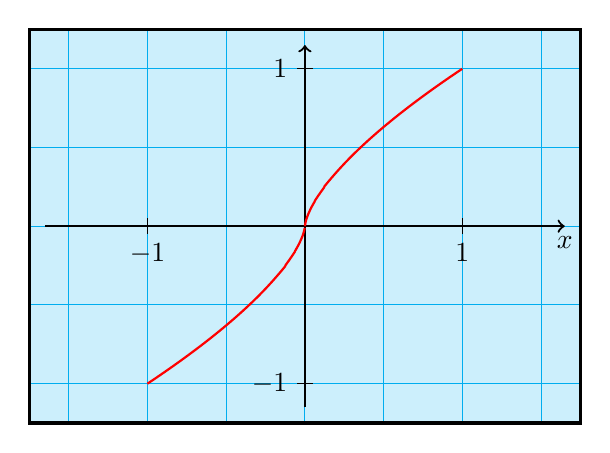
\begin{tikzpicture}
		% Hintergrund und Achsen
		\fill[cyan!20] (-3.5, -2.5) rectangle (3.5, 2.5);
		\draw[cyan] (-3.5, -2.5) grid (3.5, 2.5);
		\draw[thick, ->] (-3.3, 0) -- (3.3, 0) node[below] {$x$};
		\draw[thick, ->] (0, -2.3) -- (0, 2.3);
		\draw[thin] (-2, 0.1) -- (-2, -0.1) node[below] {$-1$};
		\draw[thin] (2, 0.1) -- (2, -0.1) node[below] {$1$};
		\draw[thin] (0.1, -2) -- (-0.1, -2) node[left] {$-1$};
		\draw[thin] (0.1, 2) -- (-0.1, 2) node[left] {$1$};
		\draw[very thick] (-3.5, -2.5) rectangle (3.5, 2.5);

		% Funktion
		\draw[thick, red] plot[smooth, domain=-2:0, samples=200] (\x, {-2*(-\x/2)^(2/3)});
		\draw[thick, red] plot[smooth, domain=0:2, samples=200] (\x, {2*(\x/2)^(2/3)});
	\end{tikzpicture}
	\caption{Illustration of minimizer $u_*$.}
\end{figure}

Clearly, $u_*\in H^1(\Omega)$ with $u_*(x)=\frac{2}{3}\lvert x\rvert^{-1/3}$, and $I(u_*)=0$. We ask: Does the first variation of $I$ in $u_*$ exist? Does $u_*$ satisfy $DI(u_*)[v]=0$ for suitable directions $v$ (e.g. $v\in C_c^\infty(\Omega)$)? We compute the derivative of $t\longmapsto I(u_*+tv)$ in $t=0$.\\

We claim that, if $v(0)\ne0$, then $I(u_*+tv)=+\infty$ for all $t\ne0$. In particular the variation in $u_*$ would not exist. Our functional $I$ splits into two integrals (one over $(-1,0)$ and one over $(0,1)$), but we only do the following calculation for the second one:
\begin{align*}
	&\int_0^1{(x^4-(x^{2/3}+tv(x))^6)^2\left\lvert\frac{2}{3}x^{-1/3}+tv'(x)\right\rvert^p\mathrm{d}x}\\
	&\qquad\qquad=\int_0^1{(x^4-x^4-6x^\frac{10}{3}tv-15x^\frac{8}{3}(tv)^2-20x^\frac{6}{3}(tv)^3-15x^\frac{4}{3}(tv)^4-6x^\frac{2}{3}(tv)^5-(tv)^6)^2}\\
	&\qquad\qquad\qquad\qquad\cdot\lvert\frac{2}{3}x^{-\frac{1}{3}}+tv'\rvert^p\mathrm{d}x\\
	&\qquad\qquad=\int_0^1{\tilde{c}t^{12}(v(x))^{12}x^{-p/3}\mathrm{d}x}+R(t),
\end{align*}
where $R(t)$ collects all lower order terms. Since $v(0)\ne0$ we have $v(x)\approx ax$ for $x\sim0$ for some constant $a\ne0$ which yields
\[\int_0^1{x^{12}x^{-p/3}\mathrm{d}x}=+\infty\]
if $p$ is sufficiently large, i.e. $12-\frac{p}{3}\leq-1$.\\[11pt]

To ensure that first variation of $I$ exists, we have to impose additional conditions on $f,\partial_Af$ and $\partial_uf$.\\

\hypertarget{theorem_3_5_2}{\textbf{\underline{Theorem 3.5.2}}}\\
(Sufficient conditions for G\^ateaux differentiability; Ren\'e G\^ateaux, * 1889, $\dagger$ 1914)\\
Let $\Omega\subset\mathbb{R}^d$ be bounded and open, and $f\in C^1(\overline{\Omega}\times\mathbb{R}^m\times\mathbb{R}^{m\times d})$ (in fact, $f\in C^0(\overline{\Omega}\times\mathbb{R}^m\times\mathbb{R}^{m\times d})$ and $f(x,\cdot,\cdot)\in C^1(\mathbb{R}^m\times\mathbb{R}^{m\times d})$ for all $x\in\overline{\Omega}$ would be enough). Let $p,q,r\in[1,\infty)$ such that $\frac{1}{r}\geq\frac{d-p}{dp}=:\frac{1}{p^*}$, $q\leq 1+\frac{r(p-1)}{p}$ and
\begin{align}
	\lvert f(x,u,A)\rvert&\leq C_1(1+\lvert u\rvert^r+\lvert A\rvert^p)\label{eq:mcov_formula_3_1},\\
	\lvert\partial_uf(x,u,A)\rvert&\leq C_2(1+\lvert u\rvert^{r-1}+\lvert A\rvert^{p-1})\label{eq:mcov_formula_3_2},\\
	\lvert\partial_Af(x,u,A)\rvert&\leq C_3(1+\lvert u\rvert^{q-1}+\lvert A\rvert^{p-1})\label{eq:mcov_formula_3_3}.
\end{align}
Then
\begin{itemize}
	\item[(i)] $I(u)\in\mathbb{R}$ for every $u\in W^{1,p}(\Omega;\mathbb{R}^m)$;
	\item[(ii)] $I$ is G\^ateaux differentiable, and for all $v\in W^{1,p}(\Omega;\mathbb{R}^m)$
	\[DI(u)[v]=\int_\Omega{\partial_Af(x,u(x),\nabla u(x)):\nabla v(x)+\partial_uf(x,u(x),\nabla u(x))\cdot v(x)\mathrm{d}x}\]
	is well-defined.
\end{itemize}

\textit{Remark: If $p>d$, we can replace $\lvert u\rvert^r,\lvert u\rvert^{r-1},\lvert u\rvert^{q-1}$ by some $b(u)$, where $b:\mathbb{R}^m\longrightarrow\mathbb{R}$ is locally bounded.}\\

\textit{Proof:}\\
The Sobolev embedding implies $W^{1,p}(\Omega;\mathbb{R}^m)\longhookrightarrow L^r(\Omega;\mathbb{R}^m)$ so that in particular it holds $\lVert v\rVert_{L^r(\Omega)}\leq C_{r,p}\lVert v\rVert_{W^{1,p}(\Omega)}$ for some $C_{r,p}>0$ and all $v\in W^{1,p}(\Omega;\mathbb{R}^m)$. Therefore, \eqref{eq:mcov_formula_3_1} gives
\begin{align*}
	\lvert I(u)\rvert&\leq\int_\Omega{\lvert f(x,u(x),\nabla u(x))\rvert\mathrm{d}x}\\
	&\leq C_1\left(\vol{\Omega}+\lVert u\rVert_{L^r(\Omega)}^r+\lVert\nabla u\rVert_{L^p(\Omega)}^p\right)<\infty
\end{align*}
for $u\in W^{1,p}(\Omega;\mathbb{R}^m)$. This shows assertion (i). For (ii), we first note that, via \eqref{eq:mcov_formula_3_2} and H\"older's inequality (and with $p'$, $r'$ being the dual exponents of $p$ and $r$, respectively),
\begin{align*}
	&\int_\Omega{\lvert\partial_uf(x,u(x),\nabla u(x))\rvert\lvert v(x)\rvert\mathrm{d}x}\\
	&\qquad\qquad\leq\int_\Omega{C_2(1+\lvert u(x)\rvert^{r-1}+\lvert\nabla u(x)\rvert^{p-1})\lvert v(x)\rvert\mathrm{d}x}\\
	&\qquad\qquad\leq C_2\left(\left(\int_\Omega{1\mathrm{d}x}\right)^{\frac{1}{p'}}\lVert v\rVert_{L^p(\Omega)}+\lVert\lvert u\rvert^{r-1}\rVert_{L^{r'}(\Omega)}\lVert v\rVert_{L^r(\Omega)}+\lVert\lvert\nabla u\rvert^{p-1}\rVert_{L^{p'}(\Omega)}\lVert v\rVert_{L^p(\Omega)}\right)\\
	&\qquad\qquad\leq C_2\left(\vol{\Omega}^{\frac{1}{p'}}+C_{r,p}\lVert u\rVert_{L^r(\Omega)}^{r-1}+\lVert\nabla u\rVert_{L^p(\Omega)}^{p-1}\right)\lVert v\rVert_{W^{1,p}(\Omega)}<\infty,
\end{align*}
since $u,v\in W^{1,p}(\Omega;\mathbb{R}^m)$. Analogously,
\begin{align*}
	&\int_\Omega{\lvert\partial_Af(x,u(x),\nabla u(x))\rvert\lvert\nabla v(x)\rvert\mathrm{d}x}\\
	&\qquad\qquad\leq\int_\Omega{C_3(1+\lvert u(x)\rvert^{q-1}+\lvert\nabla u(x)\rvert^{p-1})\lvert\nabla v(x)\rvert\mathrm{d}x}\\
	&\qquad\qquad\leq C_3\left(\vol{\Omega}^{\frac{1}{p'}}\lVert\nabla v\rVert_{L^p(\Omega)}+\lVert\lvert u\rvert^{q-1}\rVert_{L^{p'}(\Omega)}\lVert\nabla v\rVert_{L^p(\Omega)}+\lVert\lvert\nabla u\rvert^{p-1}\rVert_{L^{p'}(\Omega)}\lVert\nabla v\rVert_{L^p(\Omega)}\right)\\
	&\qquad\qquad\leq C_3\left(\vol{\Omega}^{\frac{1}{p'}}+\left(\int_\Omega{\lvert u(x)\rvert^{\frac{(q-1)p}{p-1}}\mathrm{d}x}\right)^{\frac{1}{p'}}+\lVert\nabla u\rVert_{L^p(\Omega)}^{p-1}\right)\lVert v\rVert_{W^{1,p}(\Omega)}.
\end{align*}
The condition for $q$ implies $q-1\leq\frac{r}{p'}$, i.e. $\frac{(q-1)p}{p-1}\leq r$. Thus,
\[\partial_Af(\cdot,u,\nabla u):\nabla v+\partial_uf(\cdot,u,\nabla u)\cdot v\in L^1(\Omega)\]
for all $u,v\in W^{1,p}(\Omega;\mathbb{R}^m)$. It remains to check G\^ateaux differentiability, and to this end we use the fundamental theorem of calculus: if $g\in C^1([0,1])$ then
\[g(1)-g(0)=\int_0^1{\frac{\mathrm{d}}{\mathrm{d}s}g(s)\mathrm{d}s}.\]
With that, we write the difference quotient for G\^ateaux differential. For any $t\ne0$ it holds via chain rule
\begin{align*}
	\frac{1}{t}(I(u+tv)-I(u))&=\int_\Omega{\int_0^1{\frac{1}{t}\frac{\mathrm{d}}{\mathrm{d}s}f(x,u(x)+stv(x),\nabla u(x)+st\nabla v(x))\mathrm{d}s}\mathrm{d}x}\\
	&=\int_\Omega{\int_0^1{\frac{1}{t}\partial_uf(x,u(x)+stv(x),\nabla u(x)+st\nabla v(x))\cdot tv(x)\mathrm{d}s}\mathrm{d}x}\\
	&\qquad\qquad+\int_\Omega{\int_0^1{\frac{1}{t}\partial_Af(x,u(x)+stv(x),\nabla u(x)+st\nabla v(x)):t\nabla v(x)\mathrm{d}s}\mathrm{d}x}\\
	&=\int_\Omega{\int_0^1{h(t,s,x)\mathrm{d}s}\mathrm{d}x}
\end{align*}
with $h(t,s,\cdot):=\partial_uf(\cdot,u+stv,\nabla u+st\nabla v)\cdot v+\partial_Af(\cdot,u+stv,\nabla u+st\nabla v):\nabla v$. We are interested into the limit $t\to0$, and in order to conclude we need to interchange the limit and integration. For that, we will make use of Lebesgue's dominated convergence theorem. We prove existence of a dominating function for $h$. Using the growth assumptions \eqref{eq:mcov_formula_3_2} and \eqref{eq:mcov_formula_3_3} we estimate
\begin{align*}
	\lvert h(t,s,\cdot)\rvert&\leq C_2(1+\lvert u+stv\rvert^{r-1}+\lvert\nabla u+st\nabla v\rvert^{p-1})\lvert v\rvert\\
	&\qquad\qquad+C_3(1+\lvert u+stv\rvert^{q-1}+\lvert\nabla u+st\nabla v\rvert^{p-1})\lvert\nabla v\rvert\\
	&\leq C_2\left\{1+\left(\lvert u\rvert+\lvert st\rvert\lvert v\rvert\right)^{r-1}+\left(\lvert\nabla u\rvert+\lvert st\rvert\lvert\nabla v\rvert\right)^{p-1}\right\}\lvert v\rvert\\
	&\qquad\qquad+C_3\left\{1+\left(\lvert u\rvert+\lvert st\rvert\lvert v\rvert\right)^{q-1}+\left(\lvert\nabla u\rvert+\lvert st\rvert\lvert\nabla v\rvert\right)^{p-1}\right\}\lvert\nabla v\rvert\\
	&\leq C_2\left\{1+\left(\lvert u\rvert+\lvert v\rvert\right)^{r-1}+\left(\lvert\nabla u\rvert+\lvert\nabla v\rvert\right)^{p-1}\right\}\lvert v\rvert\\
	&\qquad\qquad+C_3\left\{1+\left(\lvert u\rvert+\lvert v\rvert\right)^{q-1}+\left(\lvert\nabla u\rvert+\lvert\nabla v\rvert\right)^{p-1}\right\}\lvert\nabla v\rvert\\
	&=:\tilde{h}.
\end{align*}
So $\tilde{h}$ is an integrable dominating function for $h$ since it does not depend on $s$, $t$ (but on $x$ which is ok). Thus, Lebesgue's dominated convergence is applicable and we have
\begin{align*}
	DI(u)[v]&=\lim_{t\to0}{\frac{1}{t}(I(u+tv)-I(u))}=\lim_{t\to0}{\int_\Omega{\int_0^1{h(t,s,x)\mathrm{d}s}\mathrm{d}x}}\\
	&=\int_\Omega{\int_0^1{\lim_{t\to0}{h(t,s,x)}\mathrm{d}s}\mathrm{d}x}=\int_\Omega{\int_0^1{h(0,0,x)\mathrm{d}s}\mathrm{d}x}=\int_\Omega{h(0,0,x)\mathrm{d}x}\\
	&=\int_\Omega{\partial_Af(x,u(x),\nabla u(x)):\nabla v(x)+\partial_uf(x,u(x),\nabla u(x))\cdot v(x)\mathrm{d}x},
\end{align*}
where we have used that $h(0,s,x)=h(0,0,x)$ for all $s\in[0,1]$. We conclude that $I$ is G\^ateaux differentiable with derivative as asserted.\hfill$\blacksquare$\\[11pt]

\textbf{Corollary 3.5.3}\\
(Necessary condition)\\
If $I:u_0+W_0^{1,p}(\Omega;\mathbb{R}^m)\longrightarrow\mathbb{R}$ satisfies the assumptions of \hyperlink{theorem_3_5_2}{Theorem 3.5.2} and \hyperlink{theorem_3_4_11}{Theorem 3.4.11}, then all minimizers $u_*$ of $I$ satisfy the weak Euler-Lagrange equations, i.e., for all $v\in W_0^{1,p}(\Omega;\mathbb{R}^m)$ it holds $DI(u_*)[v]=0$. More explicitly, we have
\[\int_\Omega{\partial_Af(x,u_*(x),\nabla u_*(x)):\nabla v(x)+\partial_uf(x,u_*(x),\nabla u_*(x))\cdot v(x)\mathrm{d}x}=0\]
for all $v\in W_0^{1,p}(\Omega;\mathbb{R}^m)$, which is the weak formulation of the classical Euler-Lagrange equations
\[-\divergence{\partial_Af(\cdot,u_*,\nabla u_*)}+\partial_uf(\cdot,u_*,\nabla u_*)=0.\]\\

\textit{Remark: One can show that, if $f$ is not only convex in $A$ but also in $u$, then satisfying the weak Euler-Lagrange equations is also sufficient for being a minimizer.}\\

\textit{Proof:}\\
This follows with simple Analysis I*.\hfill$\blacksquare$\\[11pt]

\textbf{Example 3.5.4}\\
We consider
\[f(x,u,A):=\frac{\alpha(x)}{p}\lvert A\rvert^p+\frac{\beta(x)}{r}\lvert u\rvert^r,\]
where $\alpha,\beta\in L^\infty(\Omega)$, $\alpha(x)\geq\alpha_0>0$, $\beta(x)\geq\beta_0>0$ for almost all $x\in\Omega$, and $1<p<\infty$, $1<r<\infty$. The previous theorem, \hyperlink{theorem_3_5_2}{Theorem 3.5.2}, gives G\^ateaux differentiability on $W^{1,p}(\Omega)$ of
\[I(u)=\int_\Omega{\frac{\alpha(x)}{p}\lvert\nabla u(x)\rvert^p+\frac{\beta(x)}{r}\lvert u(x)\rvert^r\mathrm{d}x}\]
if $\frac{1}{r}\geq\frac{d-p}{dp}$, with directional derivative
\[DI(u)[v]=\int_\Omega{\alpha(x)\lvert\nabla u(x)\rvert^{p-2}\nabla u(x):\nabla v(x)+\beta(x)\lvert u(x)\rvert^{r-2}u(x)v(x)\mathrm{d}x}.\]
The strong form of the Euler-Lagrange equation is
\[-\divergence{\alpha\lvert\nabla u\rvert^{p-2}\nabla u}+\beta\lvert u\rvert^{r-2}u=0\quad\text{in }\Omega.\]
If $\alpha\equiv1$ then this partial differential equation is the so-called \textit{$p$-Laplacian}.